\def\rcurs{{\mbox{$\resizebox{.16in}{.08in}{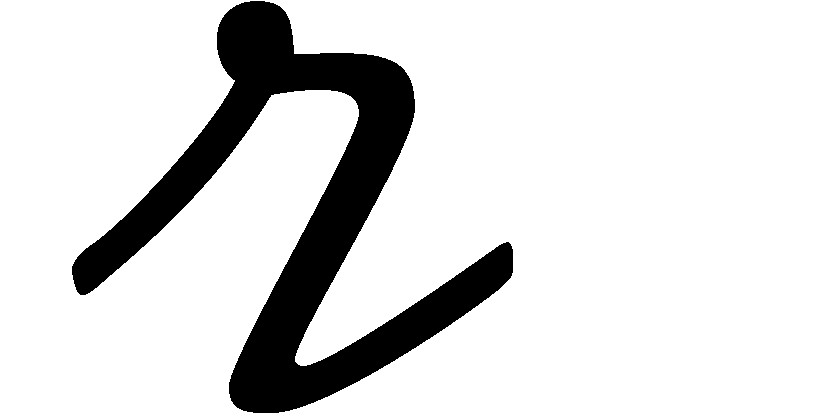
\includegraphics{ScriptR}}$}}} 

In chapters 2 and 3, Lorentz forces are discussed on individual nanoparticles. In this chapter forces between resonators are investigated, in particular a metasurface design that produces a chiral response from an array of achiral sub-structures, or meta-atoms. In general, the response of an individual meta-atom is extrapolated to explain the collective response of a metasurface, in a manner that neglects the interactions between meta-atoms. Thus, the convention is that chiral responses are born from metasurfaces composed of chiral meta-atoms. This chapter studies a metasurface that is composed of tilted achiral meta-atoms with no spatial variation of the unit-cell yet derives appreciable optical chirality solely from the asymmetric interactions between meta-atoms. Interactions between meta-atoms are modelled as the Lorentz force that arises from the Larmor radiation of adjacent plasmonic resonators because their inclusion accurately predicts the bonding/anti-bonding modes that are measured experimentally. Experimentally observed are the emergence of multiple polarization eigenmodes, among other polarization-dependent responses, which cannot be modelled with the transmission matrix formalism. The results are essential for the precise characterization and design of metasurfaces. 


\section{Introduction} 
Metamaterials are composed of sub-wavelength components, or meta-atoms that individually alter the intensity and phase of light. When placed on a 2D surface, metamaterials are known as metasurfaces [\cite{Zhao}] and have enabled many applications from quarter [\cite{Yu}], half-wave plates[\cite{Ding}], and cross-polarizers [\cite{Qin}], to ultra-thin lenses [\cite{Aieta,Ni}]. Chiral metasurfaces can ultimately be defined as those that exhibit a response dependent on the incident circular-polarization handedness, though the specific mechanism behind the phenomena has been debated; it has been argued that planar structures such as metasurfaces cannot exhibit true optical activity (OA) or circular dichroism (CD) without the excitation of magnetic resonances since certain 3D symmetry properties are not satisfied [\cite{Hentschel, Eftekhari}]. The equivalent response from planar metasurfaces can be achieved by alternate methods such as the interaction of plasmon modes [\cite{Eftekhari, Fan10}], or by non-radiative dissipation [\cite{Khanikaev}], and is named optical chirality. The difference in transmission from different polarization states due to optical chirality produces an \textit{equivalent} effect to OA and CD. 	

Optical chirality in metamaterials is produced in several ways. Not surprisingly, a chiral metamaterial can be composed of chiral meta-atoms, in which the mirror image of the structure cannot be superimposed on the original [\cite{Zhang:14, Tang2016}]. Intrinsically chiral materials are chiral due to the geometry of the meta-atoms themselves, and exhibit chiral behavior at normal illumination incidence. Helices [\cite{Kuzyk}], gammadions [\cite{Cao13, Kwon08}], or nanoparticle assemblies [\cite{FanSci, Guerrero-Martinez}] are common examples of intrinsically chiral meta-atoms that exhibit a strong chiral response. Another approach that achieves chiral asymmetry is the creation of a linear phase gradient, {\it i.e.}, illumination at oblique incidence [\cite{Yannopapas,Cao, Cao15, Cao15_2, Proscia}] or spatial variation of the unit cell [\cite{Aieta, Yu,Shaltout}]. The chiral response that arises from the linear phase gradient of either of these approaches is associated with extrinsic chirality.  

This chapter instead focuses on the optical chirality that arises solely from the interactions between achiral meta-atoms. It is postulated that the nonlinear coupling between meta-atoms originates from an interaction force derived from the Li\'{e}nard-Wiechert potential [\cite{jackson}], which accurately predicts measured changes in the experimental transmission spectra.  Rectangular plasmonic resonators are studied whose arrangement leads to chiral phenomena at normal incidence, or identical tilted achiral nanostructures in a lattice that lead to a chiral response. The individual nanostructures are achiral, yet the periodic array is chiral [\cite{Plum11, Prosvirnin}], and thus any chiral response distills the interaction between plasmonic structures. Optical chirality is expected when the lines of mirror symmetry of the nanostructures do not coincide with the lattice array \textemdash the mirror image cannot be superimposed with the original. ``Meta-optical chirality" refers to the macroscopic optical chirality that is both observed in the far-field and attributed to the interactions between plasmonic resonators.  While many have alluded to the coupling between meta-atoms [\cite{Hentschel, Hentschel:10, Metzger, Na, Rozin}], few have addressed the origin of the interaction force.  
 
Experimentally, a simple Babinet-inverted rod (dimensions $\approx \lambda/5$) is employed as the meta-atom of the metasurface and arranged in a square array. When rod-shaped nanoapertures are tilted at an angle of $22.5^\circ$ and illuminated with low-intensity visible light ($\ll 1W/cm^2$), CD is measured on the order of 0.6 degrees of ellipticity.  In comparison, while optimized and twisted split ring resonators can reach CD up to 16 degrees in the near infrared [\cite{Decker}], such meta-atoms require small features ($\approx \lambda/20$). The relatively-large dimensions of the rod nanoapertures support dipolar plasmon resonances and can be fabricated easily with robust large-area processes. An approach is demonstrated here that leverages the interactions between simpler meta-atoms in order to achieve an optical chirality.  The general approach boasts facile design, circumvents the complex structures that intrinsically chiral materials generally require, and forgoes the oblique illumination angle-of-incidence that is the crux of extrinsically chiral materials.

The chiral response exhibited by this metasurface design is both appreciable and unexpected since plasmonic interactions generally manifest as nonlinear optical responses, which require high illumination intensities [\cite{Metzger2, Kauranen}]; optical chirality are observed at intensities far below those generally required to yield nonlinear optical responses. The metasurface is interrogated with a continuum of polarization states and find that the metasurface cannot be characterized simply from its response from orthogonal circular-polarization modes.  In fact, a conventional transmission matrix description of the polarization properties is insufficient to accurately describe the optical behavior of the metasurface.  An alternative analytic representation is provided and supports a description of intensity-independent, weakly-nonlinear plasmonic limit cycles.  The model also explains why the emergence of multiple eigen-polarization modes is observed, which is also measured experimentally. The work presented in this chapter furthers the understanding of metasurface design and breaks from the long-standing convention of transmission matrices.

\begin{figure}[b!]
\centering
\includegraphics[width=\linewidth]{springs_image11.eps}
\caption{(a) Model representation: an array of plasmonic resonators (rod-shaped apertures) tilted at $\theta_s$ relative to the base of the unit meta-atom the resonators are separated into $m$- and $n$-type. The interaction force on $m$-type resonators results from the 4 nearest $n$-type resonators and vice-versa. (b) The interaction Lorentz force that arises from Larmor radiation [Eq.~\ref{eq:Fint}] for various $\theta_s$ when resonators oscillate in the $x$-direction, as a function of time. (c) The interaction force in the parallel ($x$), and perpendicular ($y$) directions when the resonators oscillate in the $x$-direction, as a function of $\theta_s$.}
\label{fig:model}
\end{figure}
 
\section{The coupling force}
In this model, the interaction between neighboring plasmonic resonators is defined as the Lorentz force produced from the oscillation of adjacent resonators. The interaction force is derived from the electromagnetic field of an accelerating charged particle given by the Li\'{e}nard-Wiechert potential [\cite{jackson}]. The force from an $m^{th}$ charge on the $n^{th}$, $\vec{F}^{int}_{mn}$, is:   
\begin{eqnarray}
 \vec{F}^{int}_{mn} = k_eq_nq_m\bigg(\frac{\hat{\rcurs}_{mn}-\vec{\beta}_n}{(1-\vec{\beta}_n\cdot\hat{\rcurs}_{mn})^3R_{mn}^2}\bigg) + \frac{k_eq_nq_m}{c}\bigg( \frac{\hat{\rcurs}_{mn}\times[(\hat{\rcurs}_{mn}-\vec{\beta}_n)\times\dot{\vec{\beta}}_n]}{(1-\vec{\beta}_n\cdot\hat{\rcurs}_{mn})^3R_{mn}}\bigg)
 \label{eq:Fint}
\end{eqnarray}
where $k_e$ is Coulomb's constant $=1/4\pi\epsilon_0$, $\epsilon_0$ is the permittivity of free space, $\vec{\beta}_{n} = \dot{\vec{r}}_n/c$, $c$ is the speed of light, $\hat{\rcurs}_{mn} = \frac{\vec{r}_m - \vec{r}_n}{|\vec{r}_m - \vec{r}_n|}$ is the unit direction from the $m^{th}$ charge to the $n^{th}$, $R_{mn}$ is the lattice distance, $q_n$ is the charge of the $n^{th}$ particle, and $\vec{r}_m, \vec{r}_n$ are the positions of the $m^{th}$, and $n^{th}$ resonator, respectively, from the origin. When the charges are stationary, Eq.~\ref{eq:Fint} collapses to the Coulomb force between two charged particles. The first term of Eq.~\ref{eq:Fint} is referred to as the ``velocity field" since it is independent of acceleration, and the second term is the ``acceleration field". With motion of the charges restricted to the 2-D plane of the metasurface, the interaction forces created by the surrounding resonators are produced in the plane of the metasurface. Though charges also oscillate in the $z$-direction, an investigation into the coupled behavior of the longitudinal fields is beyond the scope of this study. The associated Lorentz forces may explain the near-to-far-field coupling [\cite{Vuong}].

A representation of the model is shown in Fig.~\ref{fig:model}(a), in which all nanostructures are tilted by $\theta_s$ relative to the base of the unit cell. The tilt effectively restricts the direction of motion of the resonator and the interaction force is incorporated into the equations of motion for a Lorentz-Drude plasmonic resonator [\cite{Rakic}]. The metasurface is modelled such that there is no spatial variation of the unit cell, \textit{i.e.}, all nanoapertures are tilted at the angle, $\theta_s$. For analytical reasons the $x$ and $y$-axes also rotate by $\theta_s$ such that the long (short)-axis of the plasmonic resonator is always parallel with the $x$ ($y$)-axis. The $\theta_s$ determines the directions of $\vec{\beta}_m$, and $\vec{\rcurs}_{mn}$ in Eq.~\ref{eq:Fint}.
The resonators are placed in a checkerboard-like pattern of $m$- and $n$-type oscillations, and calculate the motion of each set of resonators. The second-order terms cancel by symmetry, and subsequently the interaction force between resonators scales inversely with the distance cubed. The four closest resonators provide the interaction force that couple motion in the $x$- and $y$-directions, and between $m$- and $n$-type resonators. Interaction forces from diagonal dipoles are between like-type resonators ($m$-$m$, $n$-$n$) and are neglected, in part because the increased distance between resonators reduces the interaction force, and also because the focus is on the interactions between $m$- and $n$-type. %The inclusion of interaction force from further dipoles would reduce the . 

%The interaction force [Eq.\ref{eq:Fint}] is illustrated as a function of time for various sample angles in Fig.~\ref{fig:model}(b), and as a function of sample angles, $\theta_s$, in (c), from Eq.~\ref{eq:Fint} where .
 
The total interaction force from the Larmor radiation of the four closest resonators is shown in Fig.~\ref{fig:model}(b-c), where $\beta = -i\omega x_0/c\hat{i}$ and $x_0$ is the maximum displacement of the charge oscillation, and $x_0 = 20$nm. Each resonator oscillates in the $x$-direction and produces a force in both parallel ($x$) and perpendicular ($y$) directions, $F_{\parallel}$ and  $F_{\perp}$. $F_{\parallel}$ is calculated to be approximately 20 times larger than $F_{\perp}$.
The $F_{\parallel}$ \textemdash which is always co-aligned with the long axis of the nanostructures\textemdash is maximal when the nanostructures are oriented at 0$^\circ$ or 90$^\circ$ with the edge of the unit cell. $F_{\parallel}$ couples the parallel motion between adjacent resonators in the formation of hybrid modes, which is documented in the subsequent section. When the angle of the nanostructure, $\theta_s$, is 0$^\circ$, 45$^\circ$, or 90$^\circ$, $F_\perp$ is zero, as shown in Fig.~\ref{fig:model}(b-c). These angles correspond to the lines of symmetry of the square lattice; the array is not intrinsically chiral. Alternatively, the magnitude of $F_{\perp}$ is maximized at 22.5$^\circ$, and 67.5$^\circ$ which would correspond to opposite-handed chiral structures. $F_\perp$ couples to the orthogonal dipole moment of the adjacent resonators and is the source of optical chirality in the metasurface studied, which is further documented in the following section. Though this model incorporates the Li\'{e}nard-Wiechert potential from rectangular nanostructures, the model can be generalized to model the interaction forces from arbitrary plasmonic shapes and arrays.

If the array was non-chiral there exists some combination of reflection, rotation, and translation of the nanoaperture array can be superimposed on the original. Figure~\ref{fig:chiral} illustrates that when the nanoapertures are tilted at an angle $\theta_s \neq b\times 45^\circ$ the modified array cannot be superimposed with the original, where $b$ is some integer.
\begin{figure}[th!]
\centering
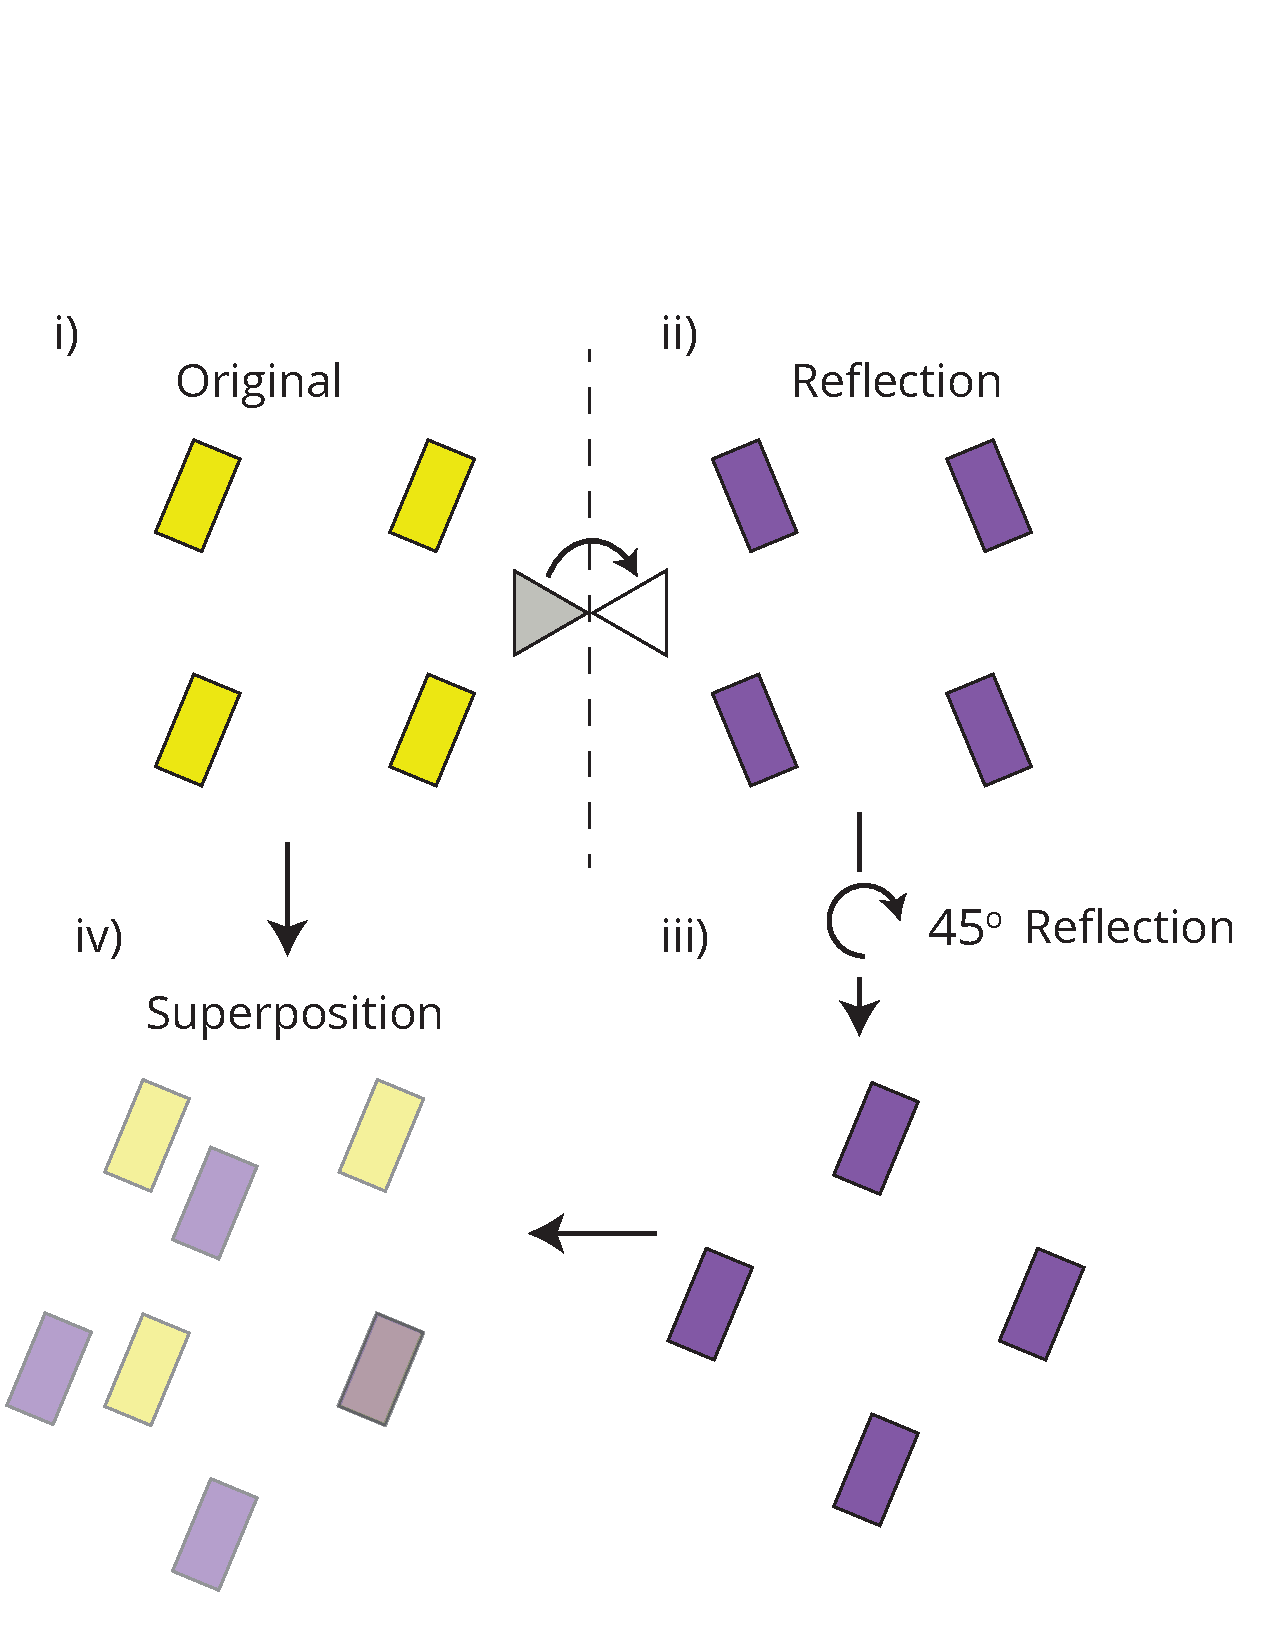
\includegraphics[width=0.9\linewidth]{chirality_proof.pdf}
\caption{(i) The original array with tilt angle, $\theta_s = 22.5^\circ$. (ii) Reflection along the vertical axis. (iii) Rotation by 45$^\circ$. (iv) Superposition of the original array with the modified array.}
\label{fig:chiral}
\end{figure}
\section{Coupled equations of motion}
The interaction force [Eq.~\ref{eq:Fint}] is summed from the four neighboring resonators to the Lorentz-Drude model and incorporate its interaction as a perturbation with the parameter, $\delta$:
$M\ddot{\vec{r}}_{m/n} = -M\omega_0^2\vec{r}_{m/n} -M\gamma\dot{\vec{r}}_{m/n}+q\vec{E}e^{-i\omega t} + \delta\sum_{n/m}  \vec{F}^{int}_{mn}$, where $r$ is the displacement of the resonator from its equilibrium position, $M$ is its mass, $\omega_0$ is the natural harmonic frequency of the resonator, $q$ is its charge, $\gamma$ is the velocity-dependent damping rate, $E_0$ is the strength of the incident driving electric field, with frequency $\omega$, subscript $m/n$ refers to the motion of either $m$- or $n$-type resonators, and dot formalism corresponds to derivatives with respect to time, $t$. 
 A separate solution is adopted for the displacement of the $m$- and $n$-type resonators shown below:
\begin{eqnarray}
x/y(t) = \frac{E_{x/y}q/M}{\omega_{0x/y}^2-i\gamma \omega-\omega^2}e^{-i\omega t} + \underbrace{x_{h}/y_{h}(t)}_\text{homogeneous solution}+ \underbrace{\delta x_{1}/\delta y_{1}(t)}_\text{perturbed solution},
\label{unperturbed_solution}
\end{eqnarray}
which includes a homogeneous solution, $x_h, y_h$, often neglected [\cite{Metzger,Metzger2,Rakic}].% An equivalent solution exists for $n$-type oscillators.
 The homogeneous solution is the general solution to the equations of motion in the absence of an external electric field and its solution is determined from the initial conditions. Even though the homogeneous solution is neglected in Optics texts [\cite{MaierBook, Levi:16, Raether:88}], it is generally present in studies of vibrations and when solving for the limit cycles of weakly nonlinear oscillators [\cite{Strogatz}]. No exact analytical solution exists for the system in which the interaction force is included; our quantitative perturbative approach employs a Taylor expansion of the interaction force, 
\begin{multline}
\vec{F}^{int}_{mn} \approx \frac{k_eq_nq_m}{R_{mn}}\Bigg[\frac{\big(\hat{\rcurs}_{mn}-\vec{\beta}_n\big)}{R_{mn}} +	 \Big(\hat{\rcurs}_{mn}\times[(\hat{\rcurs}_{mn}-\vec{\beta}_n)\times\dot{\vec{\beta}}_n]\Big)\frac{1}{c}\Bigg] \\ \times \bigg(1+3\vec{\beta}_n\cdot\hat{\rcurs}_{mn} -6(\vec{\beta}_n\cdot\hat{\rcurs}_{mn})^2-10(\vec{\beta}_n\cdot\hat{\rcurs}_{mn})^3\bigg)
 \label{eq:Fint_taylor}.
\end{multline}
%We approximate a linear relationship between the interaction force and electric field, however when the force is included into the equations of motion [Eq.~\ref{eq:Fint_taylor}], nonlinear limit cycles result.
The low-power case is considered where the transmitted polarization is independent of illumination intensity and the interaction force is linear with respect to the electric field. The system remains nonlinear because the optical response cannot be described by a superposition of incident fields. %Due to symmetry arguments, second-order electric-field terms cancel. The $\delta$ term of the perturbation analysis yields the equations of motion,
\begin{equation}
\begin{aligned}
\begin{bmatrix}\ddot{x}_{1,m}\\\ddot{y}_{1,m}\end{bmatrix} +\begin{bmatrix}
\omega_{0x}^2 & 0\\
0 & \omega_{0y}^2
\end{bmatrix} \begin{bmatrix}x_{1,m}\\y_{1,m}\end{bmatrix} +\gamma\begin{bmatrix}\dot{x}_{1,m}\\\dot{y}_{1,m}\end{bmatrix} =  \frac{1}{M}q_m\begin{bmatrix}
\kappa_{1x,n} & \kappa_{3x,n}\\
\kappa_{3y,n} & \kappa_{1y,n}
\end{bmatrix}\begin{bmatrix}E_x\\E_y\end{bmatrix},\\
\begin{bmatrix}\ddot{x}_{1,n}\\\ddot{y}_{1,n}\end{bmatrix} +\begin{bmatrix}
\omega_{0x}^2 & 0\\
0 & \omega_{0y}^2
\end{bmatrix}\begin{bmatrix}x_{1,n}\\y_{1,n}\end{bmatrix} +\gamma\begin{bmatrix}\dot{x}_{1,n}\\\dot{y}_{1,n}\end{bmatrix} =  \frac{1}{M} \underbrace{q_n\begin{bmatrix}
\kappa_{1x,m} & \kappa_{3x,m}\\
\kappa_{3y,m} & \kappa_{1y,m}
\end{bmatrix}\begin{bmatrix}E_x\\E_y\end{bmatrix}}_\text{$F^{int}$},
\label{eq:xymotion}
\end{aligned}
\end{equation}
where
\begin{multline}
\kappa_{1x} =  A_x\bigg[3k a + 2 i + 6+3k^2
\bigg(-  \langle x_{h}\rangle^2 (3ka\cos(4\theta_s)+A) \\ + \langle y_{h}\rangle^2 (9ka\cos(4\theta_s)+A)+\langle x_{h} y_{h}\rangle 9ka \sin(4\theta_s)\bigg)\bigg],
\end{multline}
\begin{multline}
\kappa_{1y} = A_y \bigg[3k a + 2 i + 6+3k^2
\bigg(  \langle y_{h}\rangle^2 (3ka\cos(4\theta_s)+A) \\ + \langle x_{h}\rangle^2 (9ka\cos(4\theta_s)+A)-\langle x_{h} y_{h}\rangle 9ka \sin(4\theta_s)\bigg)\bigg],
\end{multline}
\begin{equation}
\kappa_{3x} = 3A_xk^2
\bigg[ 3ka\sin(4\theta_s)(3\langle x_{h}\rangle^2 - \langle y_{h} \rangle^2)-3\langle x_{h} y_{h}\rangle(9ka\cos(4\theta_s)+A)\bigg],
\end{equation}
\begin{equation}
\kappa_{3y} = 3A_yk^2
\bigg[- 3ka\sin(4\theta_s)(3\langle y_{h}\rangle^2 - \langle x_{h} \rangle^2)-3\langle x_{h} y_{h}\rangle(9ka\cos(4\theta_s)+A)\bigg],
\label{kappas}
\end{equation}
and where $A_x = \frac{2k_eq_mq_nk}{Ma^2}g_{x}$, $A_y = \frac{2k_eq_mq_nk}{Ma^2}g_{y}$, $A=3ka+4i$, $a$ is the periodicity of the metasurface, $k$ is the incident wavevector, $\langle\rangle$ denotes the time-average, and $g_{x/y} =\frac{1}{\omega_{0x/y}^2-i\gamma\omega-\omega^2}$. 
 
While Eq.~\ref{eq:xymotion} may resemble a transmission-matrix formalism, the equations of motion of one type of resonator are coupled to the other by its homogeneous solution and subsequently, there are four coupled equations of motion instead of two. When the $m$-type resonators are excited, they generate Lorentz forces via the Li\'{e}nard-Wiechert potential, which contribute to both parallel and perpendicular motions of the $n$-type resonators.

The perpendicular Lorentz force couples to the orthogonal modes of the different resonators, which leads to optical chirality in the metasurface. In order to understand the terms of Eq.~\ref{kappas}, the plasmonic resonators are restricted to move only in either the $x$- or $y$-directions in the fundamental solution. The perturbative interaction becomes $\kappa_{3x/y} = \pm\frac{9k_eq_mq_n2k^4}{M a}g_{x/y}\langle y_{h}/x_{h} \rangle^2\sin(4\theta_s)$, which is zero when $\theta_s = 0^\circ, 45^\circ, 90^\circ$, \textit{etc.}, in agreement with the exact evaluation of $F^{int}$ [Fig.~\ref{fig:model}(b-c)]. Maximal optical chirality is achieved when the nanostructures are tilted at $\theta_s =$ 22.5$^\circ$ and 67.5$^\circ$. 

\begin{figure}[b!]
\centering
\includegraphics[width=\linewidth]{figure_439_wRoltLin13_wSEM.eps} 
\caption{(a) A top-view scanning electron microscope image of the metasurface. (b) The transmission spectra associated with different linear polarization angles, where the presence of bonding and anti-bonding modes is observed. (c) Shift in the wavelengths of the bonding and anti-bonding modes as a function of polarization angle. (d) Interaction forces parallel and perpendicular to the polarization axis experienced by the resonators from Eq.~\ref{eq:xymotion} as a function of polarization angle.} 
\label{fig:rotlin}
\end{figure}

\begin{figure}[b!]
\centering
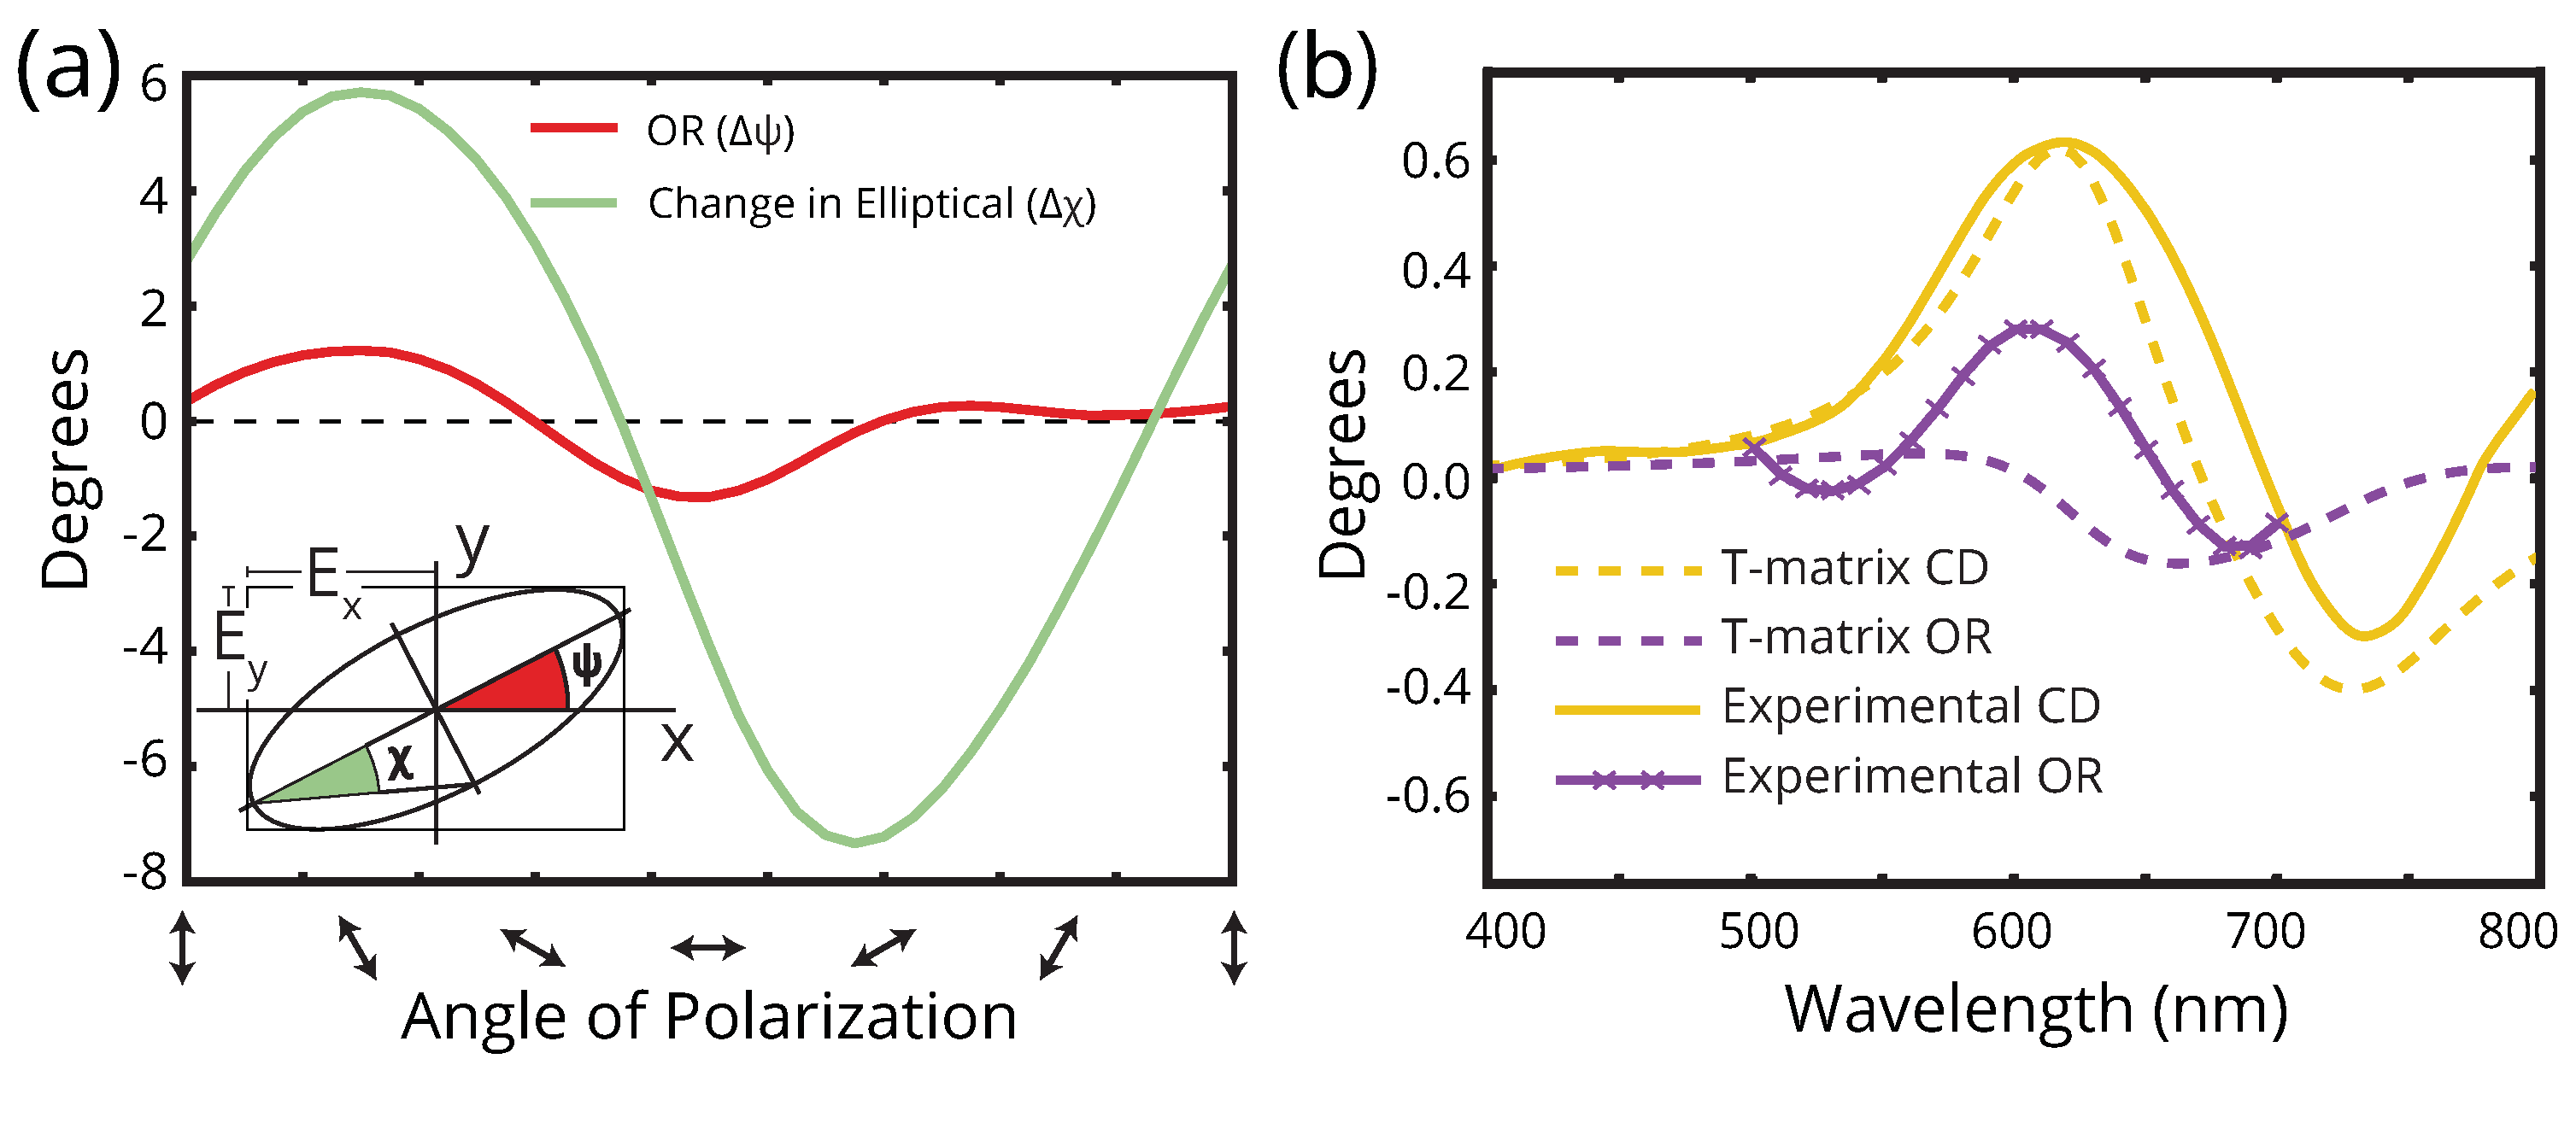
\includegraphics[width=\linewidth]{exp-OR-CD_varyPol4.eps}
\caption{(a) The optical rotation (OR) and change in the elliptical component as a function of input polarization at 660nm. Inset: the relationship between $E_x$ and $E_y$ OR and change in the elliptical on the polarization ellipse. (b) OR and circular dichroism (CD) calculated from a transmission (T-)matrix approach (dashed). Overlaid is the experimental measurements of OR (measured at $\psi=$+30$^\circ$), and the CD (solid).} 
\label{fig:CD-OR}
\end{figure} 
\section{Mode hybridization and optical chirality}
Experimentally, a metasurface is fabricated that maximizes $F_\perp$ or $\kappa_{3x/y}$ with $\theta_s = 22.5^\circ$, % We show a scanning electron micrograph of the metasurface in Fig.~\ref{fig:model}(c) 
in which rod nanoapertures are arranged on a 30-nm gold film and measure 160nm by 80nm, as shown in Fig.~\ref{fig:rotlin}(a). The periodicity, $a$, varies the relative strength of the interaction force.
A periodicity of 375nm is employed in a square array, which is small enough to observe the coupling between nanoapertures, yet large enough so that the individual responses are still present.   

The wavelength-dependent transmission properties are explored in Fig.~\ref{fig:rotlin}(b), which shows the transmission for linearly-polarized light. The axis of the illuminating linear polarization is rotated counter-clockwise from 0$^\circ$ (vertical) through 90$^\circ$ (horizontal) to 180$^\circ$ (vertical). Two absorption dips are observed in the transmission around 600nm and 730nm that correspond to the mode-splitting or mode hybridization of the plasmonic dipolar resonance [\cite{Prodan}]. 
The spectral locations of the bonding and anti-bonding modes correspond to the mode coupling or interaction force $F^{int}$. When the periodicity decreases, $F^{int}$ increases and the resonances separate further; if the separation between meta-atoms increases, then the transmission resonances collapse to the transmission profile of a single resonator [\cite{Prodan}]. The trends associated with meta-atom spacing indicate that the transmission dips observed are not a Wood's anomaly grating effect, which is related to lattice absorption. Wood's anomaly resonances would scale in proportion with the metasurface spacing. Moreover, Wood's anomalies are characterized by ultrasharp resonances [\cite{Yang16}] which are not observed. 

The parallel component of the interaction force leads to the mode-splitting in the metasurface. The spectral difference between the bonding and anti-bonding modes is shown in Fig.~\ref{fig:rotlin}(c) with a Savitzky-Golay filter [\cite{Savgol}] overlaid. The interaction force is evaluated in the approximation [Eq. \ref{eq:xymotion}] in order to relate the model to the mode splitting. The components of the interaction force, $F_{\perp}$, $F_{\parallel}$, and $|F| = \sqrt{F_{\perp}^2+F_{\parallel}^2}$ are shown in Fig.~\ref{fig:rotlin}(d), where the input polarization is rotated from 0$^\circ$ to 180$^\circ$. The $F_{||}$ and the trendline of the spectral shift both exhibit maximal values between 45$^\circ$ and 55$^\circ$, where the illuminating linear polarization connects opposite ends of vertically-adjacent resonators.  The minimal values of the spectral splitting occur between 135$^\circ$ and 145$^\circ$ and correspond with an angle where the illuminating linear polarization connects opposite ends of horizontally-adjacent resonators.  Differences between the model and experiment result from the fact that in the model, only $20$nm resonator displacement is considered whereas in experiment, the effective resonator dipole is the length of the nanorod, or $180$nm. Moreover, the approximation of $F^{int}$ only accounts for the four nearest resonators and incorporates only time-harmonic terms.  Nevertheless, the strength of the parallel force $F_{||}$ scales approximately with the experimentally-measured spectral splitting of transmission resonances. 
 
The interaction force leads to other experimentally-measured polarization-dependent metasurface responses.  
The metasurface is illuminated with linearly-polarized light (ellipticity $\chi< 1 ^\circ$) at a wavelength $\lambda = 660$nm and observe that the transmitted changes in the azimuthal and elliptical components of the fields, $\Delta \psi$ and $\Delta \chi$, depend on the angle of linear polarization [Fig.~\ref{fig:CD-OR}(a)]. The change in azimuth $\Delta \psi$ denotes optical rotation (OR) and the change in the elliptical component $\Delta \chi$ denotes the phase accumulation between the $E_x$ and $E_y$-components. When the illuminating polarization angle rotates a full revolution, the trendline for the OR exhibits 4 inflection points. The OR and the perpendicular interaction force $F_\perp$ follow a similar trend [Fig.~\ref{fig:rotlin}(d)], which is expected since $F_\perp$ is the source of the optical chirality in our metasurface.  

Optical chirality is conventionally determined by the off-diagonal elements of transmission matrix of the metasurface  [\cite{Wu16, Plum14,Plum11}] but there are limits to this transmission matrix formalism. The polarization density of the material is calculated with the relation $\vec{P} = N_0q\vec{r}$, where $N_0$ is the free charge carrier concentration of the material, $q$ is the charge of the particles, and $\vec{r}$ is the direction and subsequently:
$\vec{P} = N_0q\begin{bmatrix}
x_0+x_1\\y_0+y_1
\end{bmatrix} = \epsilon_0(\epsilon-1)\vec{E}(\omega, r)+\Gamma(\nabla\times\vec{E}(\omega,r))$, and the non-locality parameter, $\Gamma_{x/y} = \frac{iN_0q_mq_n\kappa_{3x/y}}{k(\omega_{0x/y}^2-i\gamma\omega-\omega^2)}$, and $\Gamma$ is the mean of $\Gamma_x$ and $\Gamma_y$. The relations for OR$ =\frac{\omega}{2c}\Re(\Gamma) $, and CD$ = \frac{2\omega}{c}\Im(\Gamma)$, are shown as a function of the incident wavelength for tilt angle of $\theta_s = 22.5^\circ$ in Fig~\ref{fig:CD-OR}(b) and the experimental observation is overlaid. The CD is defined as the differential circular-polarization absorption as CD$(^o) = (T_{RCP}-T_{LCP})\times 32.982^\circ$ in degrees of ellipticity [\cite{Barron}]. The experimental results for CD qualitatively agree well with the analytical theory for the CD, where peaks in CD are present at both dipolar modes. In a transmission-matrix calculation, there is less agreement between the real component of $\Gamma$ and the experimentally-measured OR. It is expected that CD may be more accurately modeled with transmission matrices because the rotating circular polarization averages all linear-polarization responses, and reduces the polarization-dependence illustrated in Fig. \ref{fig:rotlin}. The discrepancies between theoretical and experimental OR indicate the limit of the transmission matrix formalism that assumes that all resonators oscillate in-phase, which may not be true when an interaction force is present between meta-atoms.

\section{Emergent polarization eigenmodes}

\begin{figure}[b!]
\centering
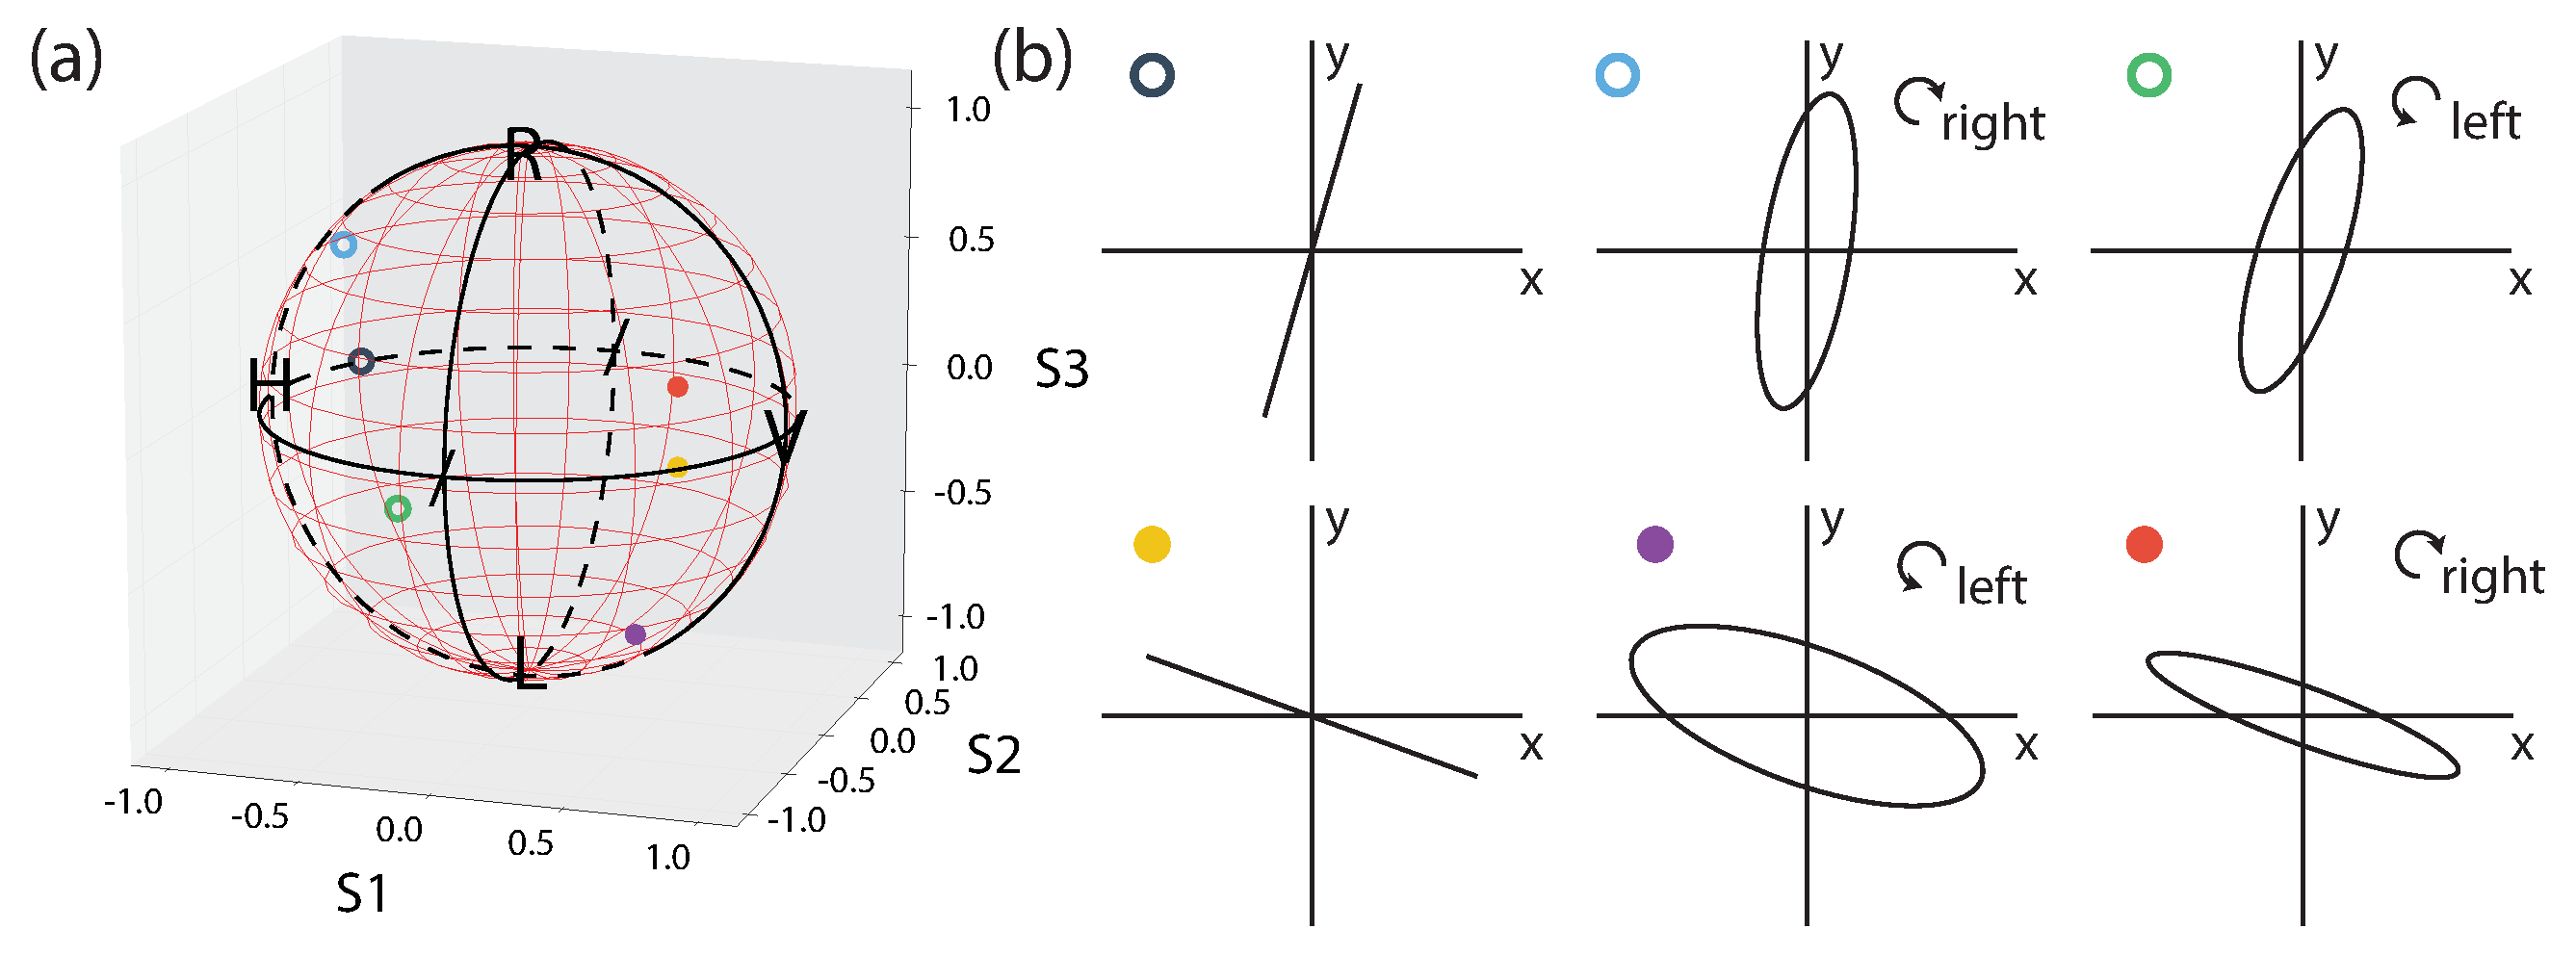
\includegraphics[width=\linewidth]{fig-eigPols-eps-converted-to.pdf}
\caption{Eigen-polarization modes of the system at 660nm are shown on (a), the Poincar\'{e} sphere, where solid circles represent eigen-polarization states on the near surface of the sphere and hollow circles represent states on the far surface. (b) illustrates the eigen-polarization states measured in the $x-y$ plane.}  
\label{fig:eigenpolarizations} 
\end{figure}

The metasurface is interrogated with a continuum of polarization states and observe polarization-dependent responses other than OR that cannot be recreated by transmission matrices. The properties of the metasurface eigen-polarization modes are characterized at a wavelength of 660nm on the Poincar\'{e} sphere [Fig.~\ref{fig:eigenpolarizations}(a)]. Figure~\ref{fig:eigenpolarizations}(b) shows the eigen-polarization modes mapped onto the $x-y$ plane, where the wave travels in the $z$-direction. The eigen-polarization modes of the system are interpreted as eigenmodes of the coupled equations of motion of the system.

Six eigen-polarization modes of the metasurface are measured, where a standard transmission matrix approach asserts the existence of only two [\cite{Gevorgyan}]. Two of the six eigen-polarization modes are approximately linearly-polarized, and the remaining four are elliptically-polarized. The presence of the multiple eigen-polarization modes cannot be characterized by the conventional, single transmission matrix formulation \textemdash which assumes that adjacent resonators are excited in phase \textemdash and supports an alternative model of coupled resonators. 


There is potentially a misconception that transmission matrices should describe any metasurface optical response that is independent of the illumination intensity. The optical response from this metasurface is linear because the transmitted polarization does not change with illumination intensity and would not produce the prototypical nonlinear optical response, for example, higher-harmonic generation, particularly at low illumination intensities. At the same time, the transmitted polarization from our metasurface is nonlinear in a manner that the optical response cannot be described by a superposition of incident fields. It appears insufficient to characterize the polarization properties of the metasurface by deriving a transmission matrix from the optical response of select linear or orthogonal circular polarizations. The corresponding system of equations in the model predicts multiple polarization eigenmodes that are observed at visible wavelengths and at low illumination power, independent of illumination intensity.

\section{Discussion}

The inclusion of an interaction force leads to responses that are not predicted via transmission matrices, such as polarization-dependent OR or multiple eigen-polarization modes, which are measured in this investigation. Discrepancies from a transmission matrix formalism may be minimal when the interaction force is small and when meta-atoms are separated significantly far apart [\cite{Haus}]. However, initial calculations suggest that the Larmor radiation from adjacent meta-atoms achieves intensities comparable to that of the incident electric field, even at low illumination intensities, due to the strong acceleration of charges on sub-wavelength nanostructures at visible wavelengths. Moreover, the constructive interference of Larmor fields in periodic lattice structures such as metasurfaces is measurable. The Larmor radiation field may be engineered to produce a desired electromagnetic response.
One method to increase the Larmor radiation, and thus the optical chirality, is to reduce the periodicity of the nanostructures since the interaction force [Eq.~\ref{eq:Fint}] scales with the inverse distance between resonators. However, as \cite{Lee16} showed, the dependence on periodicity does not continue to increase the interactions forces indefinitely since at the limit of zero periodicity the scattering cross section of the array of coupled plasmonic resonators is expected to reduce to that of a single resonator. In order to satisfy this condition, a screening factor of $ S=1-e^{-\sqrt{2/3}ka}$ is employed so that the interaction forces converge to zero at zero periodicity.  

\section{Conclusion}
In conclusion this chapter proposes a facile design approach to achieve optical chirality at normal incidence in planar arrays of achiral nanoapertures that leverages the interaction force between coupled resonators. Optical chirality results from perpendicular Lorentz forces associated with the Li\'{e}nard-Wiechert potentials when plasmonic resonators are sufficiently close. Bonding/anti-bonding modes observed in the transmission spectra result from the parallel components of the interaction forces. The polarization properties are studied and it is demonstrated that this metasurface exhibits both OR and CD equivalent responses at normal incidence in the visible regime, a property found only in chiral materials. The OR depends on the incident angle of polarization and cannot be fully described by transmission matrices. This principle is futher demonstrated through the measurements of several eigen-polarization modes. The presence of appreciable optical chirality in our metasurface indicate Larmor radiation plays a significant role in the polarization properties of metasurfaces.

\section{Fabrication methods and measurement}
\par The device can be fabricated by depositing a nanopatterned gold layer onto an ohmic conductor. The gold layer can be deposited onto the ohmic contact via thermal deposition which can give accurate layer thicknesses. Layer thicknesses are determined using a Filmetrics spectral reflectance analyzer. A calibration layer is first deposited on a substrate to correctly determine the rate of deposition for particular equipment settings. Once the rate of the metal are determined, the layer can be deposited, and the layer thicknesses determined using the spectral reflectance analyzer. Following, a layer of high resolution positive electron beam resist, ZEP-520A, is spin-coated on the gold layer. ZEP-520A is required to show the sharp definitions and high resolution that the nanostructure design demands. The nanostructure is patterned into the ZEP-520A resist using electron beam lithography, using ion beam milling the patterned resist is removed and gold where the the resist was etched away. This process can achieve either gold nanostructures or a gold film with nanoapertures. 

%Alternatively, the bottom contact of the device could be made of TCO-coated glass, much like the top contact [Fig. \ref{Schem}b]. This would increase efficiency by allowing photons to generate electron hole pairs directing in the semiconductor layer, however costs increase due to the high cost of TCO over non-transparent, opaque, conducting contacts such as metals.\par
%Another approach to plasmonic excitation in the plasmonic layer is to use a Babinet-inverted structure, in which the nanostructures are replaced with a gold film with apertures the same shape as the nanostructure~\cite{bornwolf,Hentschel}.\\
%\begin{figure}[h!t]
%\centering
%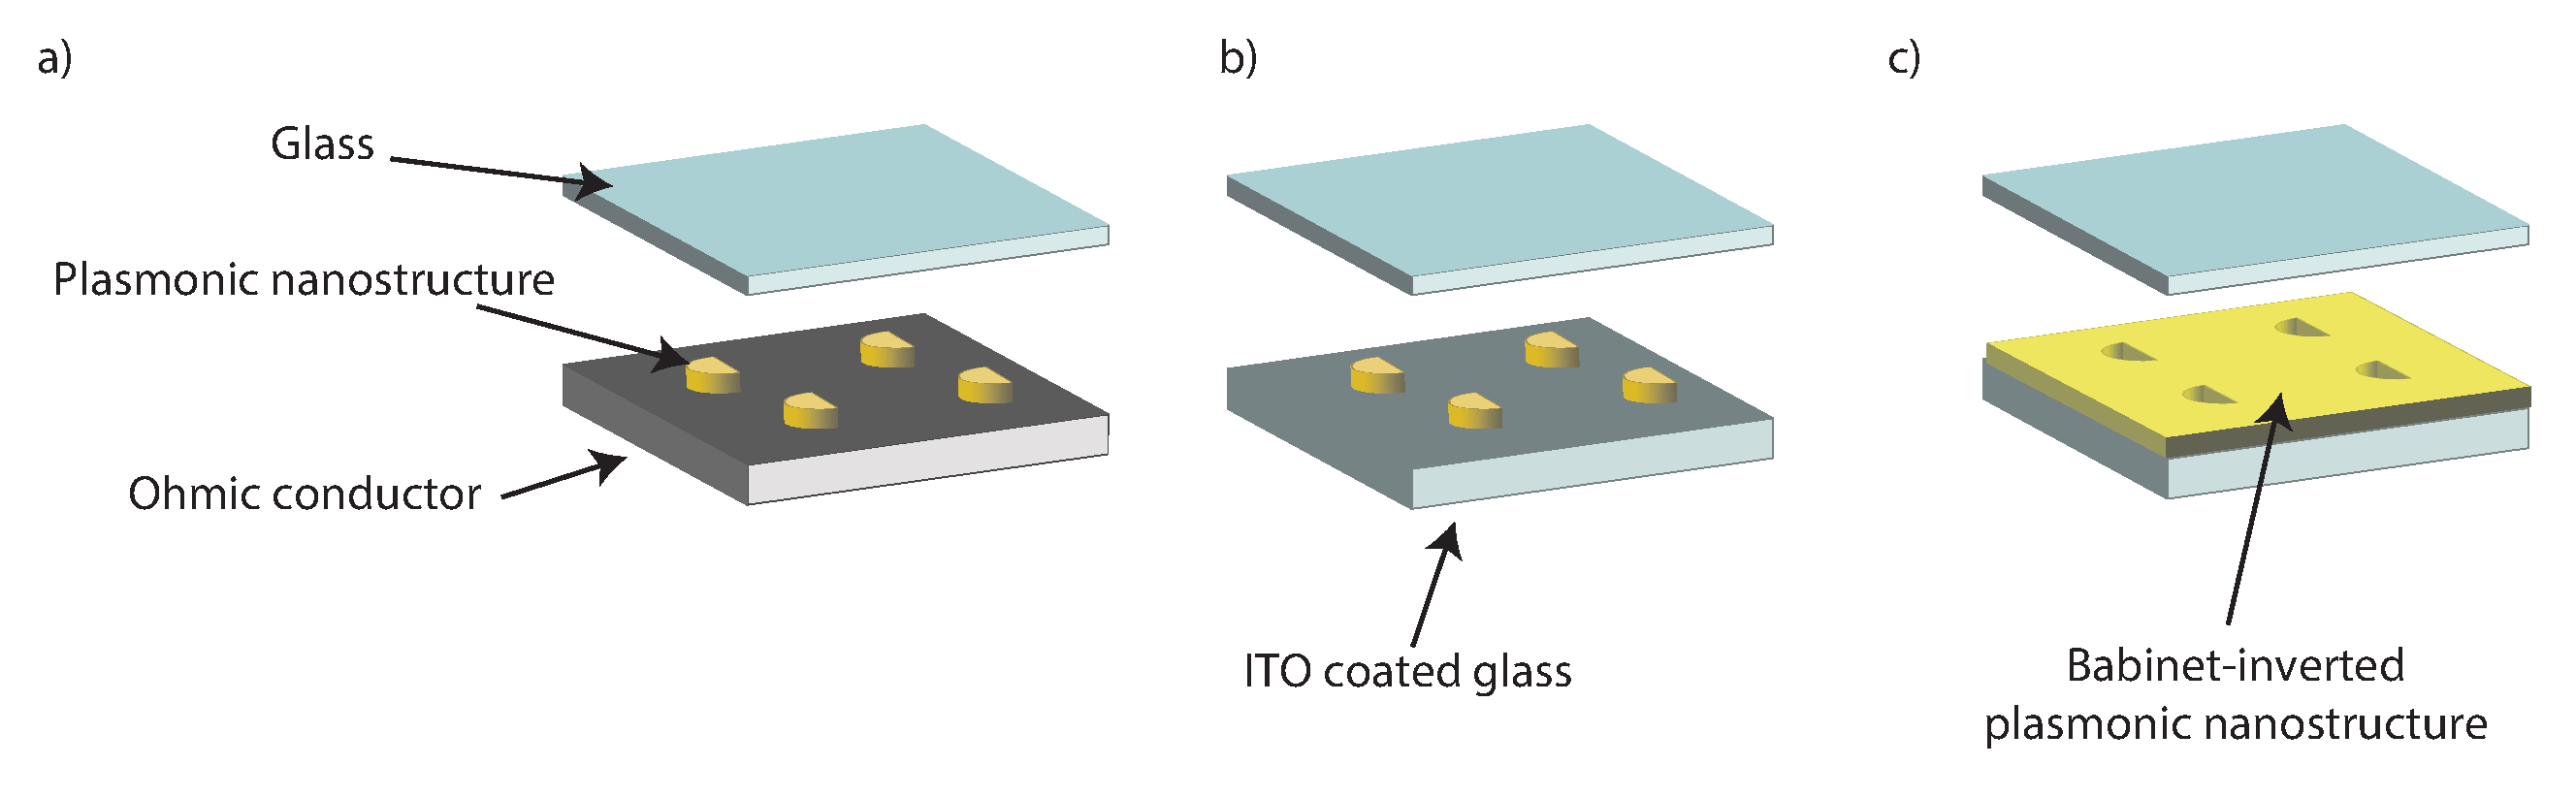
\includegraphics[width=\textwidth]{3Schem2.pdf}
%\caption{Device schematic}
%\label{Schem}
%\end{figure}
\par The patterns are created in Adobe Illustrator since the dimensions of the objects are accurately input. Adobe Illustrator also has the feature of exporting to DXF and DWG files. These files are compatible with the BEAMER software that is provided at Brookhaven National Lab to create the patterns compatible with the electron beam lithography machine.
\begin{figure}[h!]
\centering
\tikz[baseline=(a.north)]\node[yscale=-1,inner sep=0,outer sep=0](a){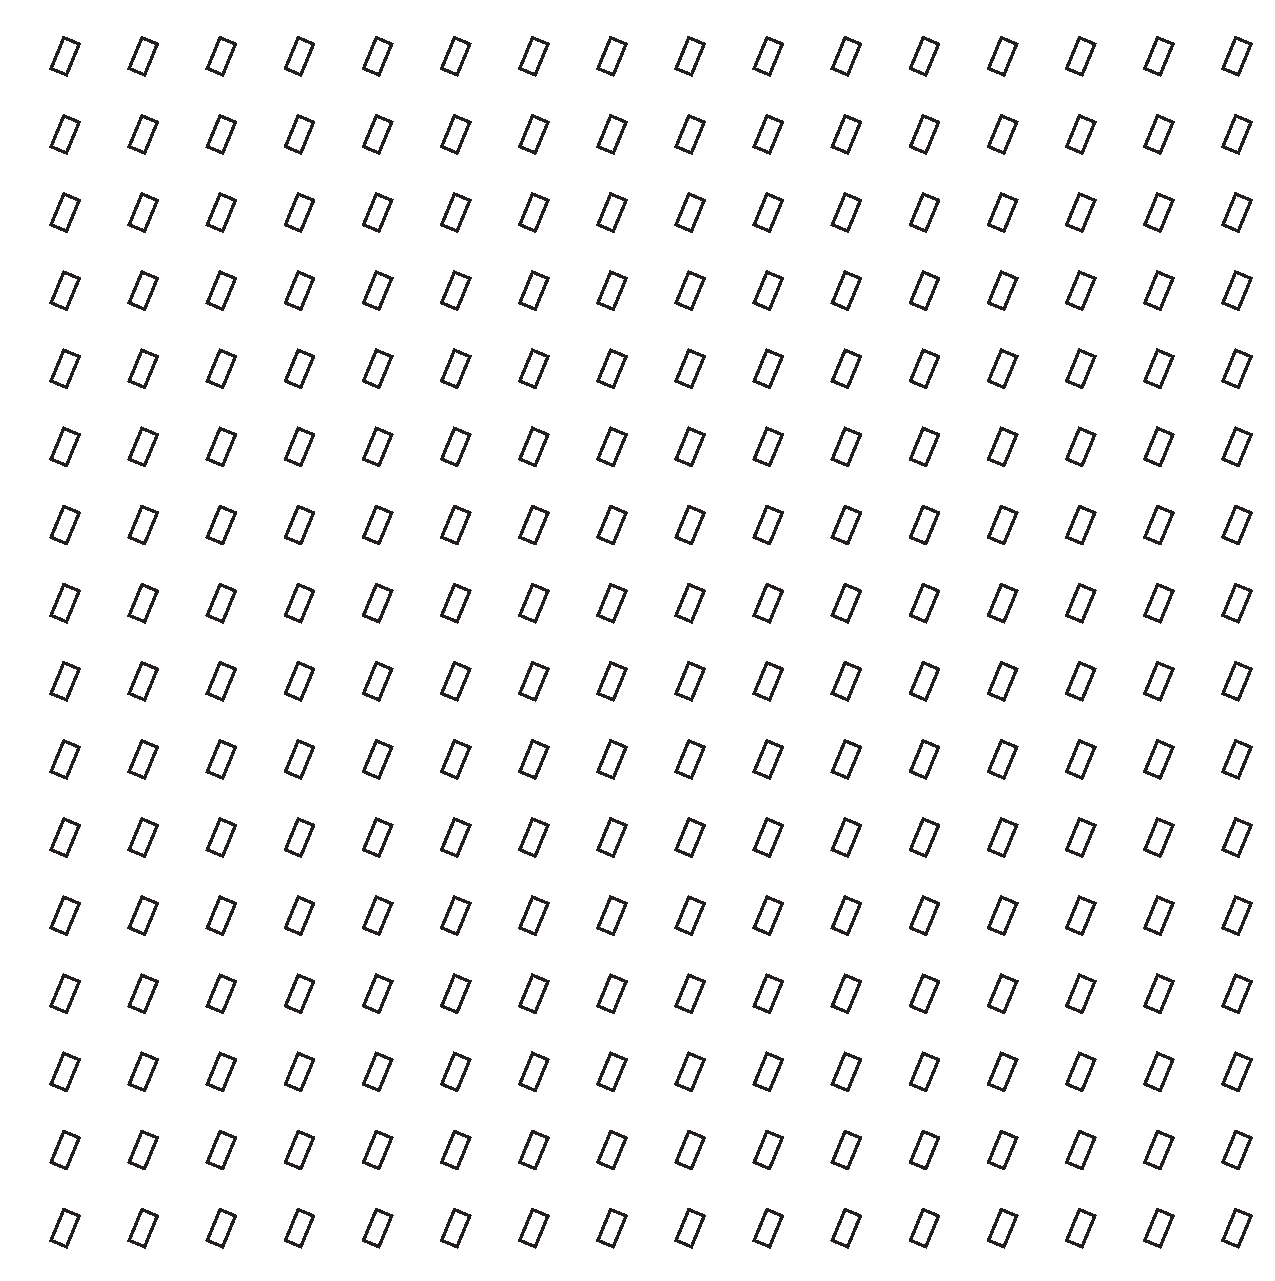
\includegraphics[width=0.75\textwidth, angle = 90]{ApertureRodDesign.pdf}};
\caption{Electron beam lithography pattern, nanoapertures measure 80nm by 160nm in a square lattice with periodicity between the structures measuring 375nm.}
\label{EbeamPattern}
\end{figure}
\subsection{Development}
\subsubsection{Electron beam resist}
The electron beam resist used was ZEP-520A, the resist thicknesses as a function of spin speed and dilution has been studied elsewhere [\cite{SpinCurve}], the thickness data is given as follows in Fig. ~\ref{spinCurve}. ZEP-520A has the properties of showing very high resolution. This is important for this work since the structures that will fabricated are on the order of 10$^{-8}$m (10nm), and thus the electron beam resist needs to show the greatest contrast for the nanostuctures to be well defined and have the desired optical properties. 

Another common electron beam resist that was considered is PMMA. PMMA is the most common electron beam resist used since it offers high resolution, is easy to handle and film characteristics have been well-studied. Though, like ZEP-520A, PMMA also provides high resolution it exhibits low contrast, which could lead to undesired optical properties.

Characteristics of ZEP-520A, are that it has a positive tone, resolution of at least 20nm, has a dry etch resistance similar to many photo resists. The film life, however is relatively short compared to other electron-beam resists such as PMMA.
\begin{figure}[h!]
\centering
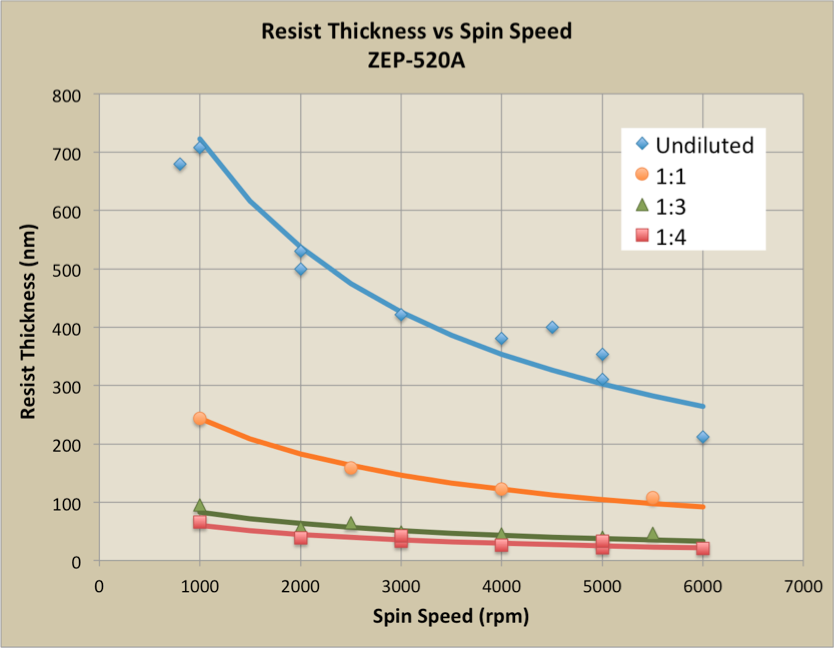
\includegraphics[width=0.75\textwidth]{ZEP520a_spincurve.png}
\caption{Spin curve for ZEP-520A. \\Image: https://ebeam.mff.uw.edu/ebeamweb/process/ process/zep520a.html}
\label{spinCurve}
\end{figure}
\subsubsection{Fracturing}
The shot pitch of the electron beam lithography machine is set to 0.125nm. Since at some points of the structure the shot pitch is not exactly divisible by the shape size, the dimensions of the shape produced may be slightly off (by a maximum of one shot pitch)  To solve this problem shot pitch fracturing is enabled, such that some extra pixels are overlapped and the correct dimensions specified are achieved [\cite{BEAMER}]. This is important in fabricating the structures since they have very small feature sizes. Plasmonic effects are highly sensitive to structure dimensions, thus, shot pitch fracture is necessary to retain the specific dimensions of the nanostructures, and by relation the plasmonic response is preserved.
\subsubsection{Proximity effect correction}
Electron beam lithography can often make sharp corners rounded. The reason for this is due to scattering of the electron beam in the resist and substrate leading to undesired resist etching in the proximity of the beam, known as the proximity effect [\cite{PEC}]. Though the individual shapes are the same size the edges of nanostructures are likely to experience the proximity effect.

One way to use proximity effect correction is via dose modulation, in which each individual shape in a pattern is given a dose such that the shape prints the correct size. Generally, the proximity effect can be thought of as larger-patterned areas receive larger doses due to the electron scattering. To compensate the larger areas receive slightly lower dosages, or alternatively, the smaller areas receive slightly higher dosages.

Another method to resolve the proximity effect is via pattern biasing. In this method the larger dose that greater area patterns receive from the proximity effect is compensated by making the area either smaller or less dense. 

%\begin{figure}[h!]
%\centering
%\includegraphics[width=0.5\textwidth]{EBeamPattern2.png}
%\caption{Electron beam lithography pattern}
%\label{EbeamPattern2}
%\end{figure}
\subsubsection{Developers}
There are a number of different developers available for use. Xylenes are a common developer since the dosage needed is low, so patterns can be written faster, however the contrast is generally low. Amyl-acetate has a higher contrast, and hexyl-acetate has the highest contrast. Though the higher the contrast, the higher dosage generally needed to write the pattern and develop effectively. Contrast can b further improved by developing at low temperature.\\

\subsection{Recipe}
The recipe of rod-shaped nanoapertures is as follows:
First on a glass substrate a 3-nm wetting layer of chromium was deposited, followed by a 30-nm layer of gold with an electron beam evaporator. The thicknesses of the layers were accurately measured via a Filmetrics F20-UV thin film analyzer. From an initial test sample the rates of the electron beam evaporator were accurately determined to produce reliable film thicknesses. The rates of chromium and gold were deposited at a rate of 0.4$\AA$ per second to produce film with high uniformity and low surface roughness($<$2nm).

Next a layer of ZEP 520a is spin-coated onto the sample. The thickness of which is determined by the thickness of gold and the ion-milling rates of both gold and ZEP 520a. Since the desired result is a gold film with rod-shaped apertures that propagate the entire thickness of the film, once the pattern is written on the resist, and developed, there will be rod-shaped apertures in the resist. At the ion-milling stage, where the pattern is written gold is exposed to the ion miller and will be milled away, everywhere else only the resist is exposed to the ion miller and will be milled. Ideally, as the resist is milled away, and the gold is milled away where the pattern is written, once the entire layer of resist is completely milled away, so is the gold, where the pattern is written. Therefore the layer of resist that needs to be spin-coated is equal to:
\begin{equation}
L_{ZEP} = \frac{MR_{Au}}{MR_{ZEP}}\times L_{Au},
\end{equation}
where $MR_{AU}$ is the milling rate of gold, $MR_{ZEP}$ is the milling rate of the resist, ZEP 520a, $L_{Au}$ is the layer thickness of gold, and $L_{ZEP}$ is the layer thickness of ZEP 520a.

Using test samples of substrates with gold and spin-coated ZEP 520a, by measuring the thicknesses of the respective layers both before and after a specified time of ion-milling, the milling rates for both gold and ZEP 520a were determined to be approximately 0.1$\AA/s$ and 1.0$\AA/s$ respectively. With a gold layer thickness of 30nm, the layer of ZEP 520a that was spin-coated necessarily had to be at least 300nm. In this way, in the ion milling process the layer of resist will be completely milled away at the same time that the gold will be milled away where the pattern is written. Fig.~\ref{spinCurve} shows that for a 1:1 dilution of ZEP 520a the spin speed should be approximately around 500rpm for the desired 300nm film thickness.
\begin{figure}[h!]
\centering
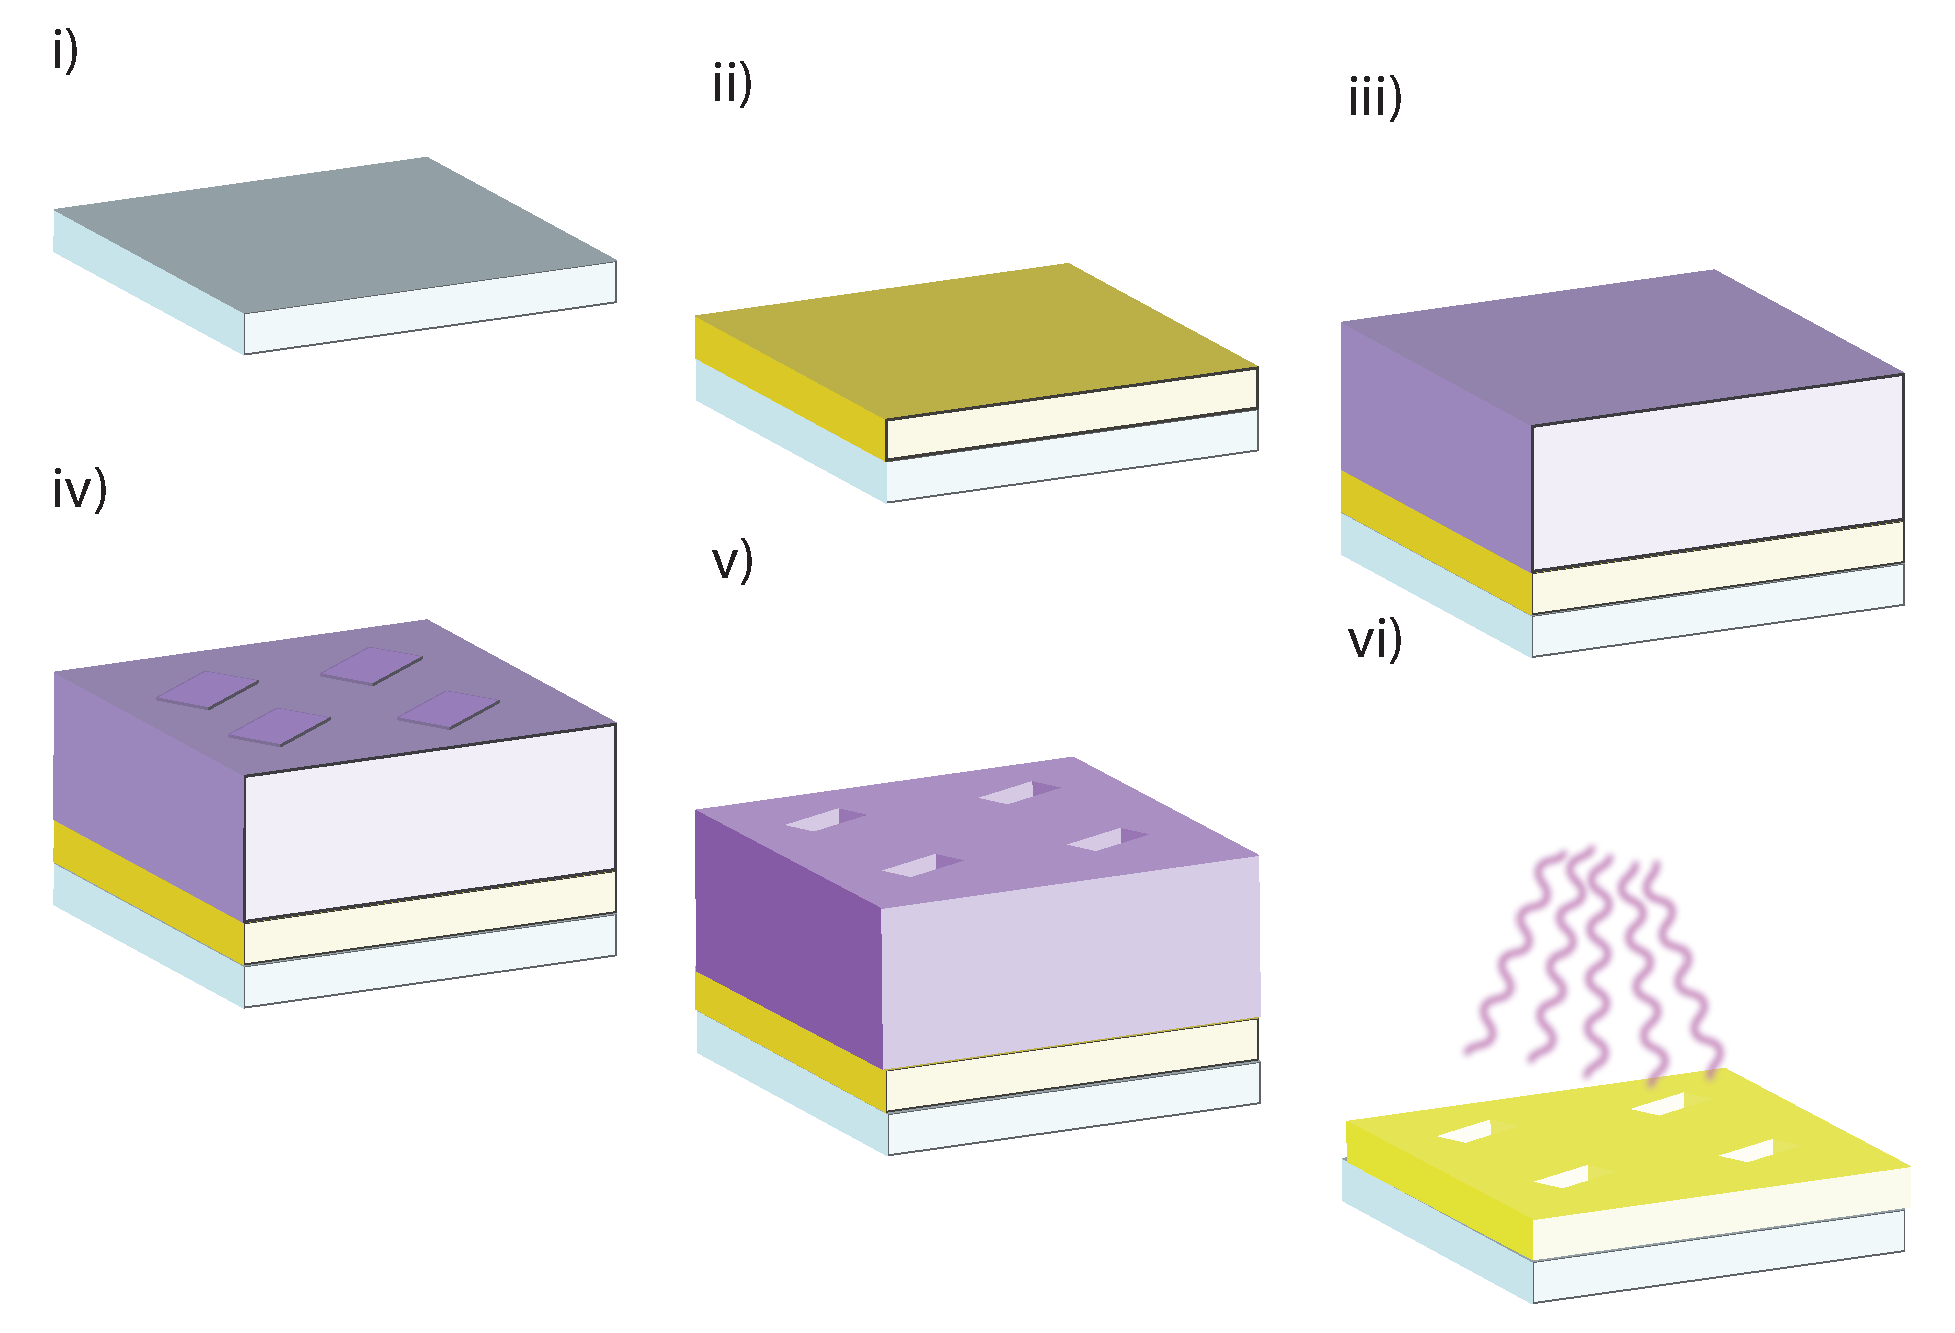
\includegraphics[width=0.9\textwidth]{NanoApertureRecipeRods.pdf}
\caption{Recipe to fabricate nanoapertures. i) Glass substrate, ii) gold layer is deposited, iii) ZEP 520a electron beam resist is deposited, iv) pattern is written via electron beam lithography, v) pattern is developed, vi) resist and gold is milled away}
\label{NanoApertureRecipe}
\end{figure}

Following, a 1.5mm $\times$ 1.5mm area pattern is written on the resist with the electron beam lithography machine. A via trial-and-error a dosage of $500\mu C/cm^2$ was used. Trial-and-error was performed by setting a variety of dosages, running the pattern, developing, and inspecting under a scanning electron microscope to determine which particular dosages were under/over-exposed, and which worked best. In the same way the current of the electron beam was determined to be 250pA.% on mode 6. Lower currents allowed for smaller patterns to be written which was needed for the smaller feature sizes and 250pA is a relatively small current. Mode 6 is used opposed to mode 3 for the smaller allowed shot pitch, 0.125nm for mode 6, opposed to 2nm for mode 3. Before each pattern is written the machine is calibrated to ensure the machine is optimal.\\

Once the pattern is written the sample was developed, hexyl-acetate was determined to be the best developer due to its high contrast especially at low temperature conditions. The sample was developed in hexyl-acetate at -25$^oC$ in a propylene glycol bath for 90 seconds followed by a rinse in iso-propyl alcohol.\\
Finally the sample was ion-milled such that the remainder of the resist is removed. The sample was visually inspected for any resist. The resulting metasurface is shown in Fig.~\ref{fig:rotlin}(a) as a scanning electron microscope image viewed from above. 
\begin{figure}[t!]
\centering
\includegraphics[width=0.7\linewidth]{bothSchem.eps}
\caption{The schematic diagram for (a) transmission measurements and (b) polarization measurements.}  
\label{fig:schematics} 
\end{figure}
\subsection{Transmission measurement setup}
To measure the optical chirality from the metasurface a xenon solar simulator is employed that provides stable broadband illumination between 400nm and 1000nm. The polarization state of light is controlled with a wire grid polarizer a 400-nm to 800-nm achromatic quarter-wave plate. The spectrum from the sample is captured via a CCD-coupled spectrometer [Fig.~\ref{fig:schematics}(a)].  

\subsection{Polarization measurement setup}
The eigen-polarization states are determined in a similar setup described above, however a spectral filter is used and the CCD-coupled spectrometer is replaced with a polarimeter to determine the polarization of transmitted light [Fig.~\ref{fig:schematics}(b)].

\section{Experimental difficulties and future work}
It has been demonstrated that chiral phenomena exists in regular arrays of rod-shaped nanoapertures tilted at 22.5$^\circ$. To further establish this phenomena, arrays of nanoapertures may be fabricated with varying tilt angles and periodicities. Variation of the periodicity would affect the coupling between nanostructures, and variation of the tilt angle would vary the strength of the perpendicular force generated that leads to the chiral phenomena observed.

The same effect may also be achieved with nanostructures, i.e., the non Babinet-inverted structure. The recipe for this type of metasurface was attempted however, due to the lift-off step, which can be quite difficult to perform, this type of metasurface was not pursued. The type of metasurface is fabricated in much the same manner as the one investigated, however the gold film is deposited after the electron beam lithography process. This makes the fabrication challenging as the non-conductive property of the glass substrate creates a difficult environment to perform the electron beam lithography.

Future work may also involve exploration into the optical forces that arise with the chiral phenomena, named optical rectification. Transverse Lorentz forces arise when light is illuminated on the metasurface [\cite{Proscia}] that are realised as a transverse voltage which are theoretically measurable on this metasurface. Moreover due to the non-centrosymmetric pattern that the rod-shaped nanoapertures exhibit when tilted at angles such as that studied here, $\theta_s=22.5^\circ$, the transverse voltages should exist even at normal incidence. These measurements typically require intense pulsed laser fields ($>$1MW/cm$^2$) and sensitive voltage measurement instruments.

Preliminary work was performed in the area of chiral responses and transverse voltages from other shapes, namely semi-circles or D-shapes. These shapes differ from the rectangular, rod-shapes studied here in that the the fundamental shape is non-centrosymmetrical, the shape can only can only be superimposed in rotation of $n\times 2\pi$ radians, where $n$ is an integer. The rod-shapes however are identical when rotated by $n\times \pi$ radians. Arrays of both shapes, when placed in an array cannot be titled at an angle $m\times \pi/4$ radians, where $m$ is integers including 0, otherwise symmetry is not broken. If the shapes are tilted prescribed by the condition above chiral phenomena occurs at normal incidence. The phenomena is much weaker in magnitude at normal incidence than structures optimized for oblique incidence but serves a much more general method to achieve chiral phenomena in metasurfaces. 